
\documentclass[a4paper,12pt]{article}
\usepackage[utf8]{inputenc}
\usepackage[a4paper,
            bindingoffset=0.2in,
            left=1in,
            right=1in,
            top=1in,
            bottom=1in,
            footskip=.25in]{geometry}


%###############################################################################

%\input{~/layout/global_layout}


%###############################################################################

% packages begin

\usepackage[
  backend=biber,
  sortcites=true,
  style=alphabetic,
  eprint=true,
  backref=true
]{biblatex}
\addbibresource{bibliography.bib}

\usepackage{euscript}[mathcal]
% e.g. \mathcal{A} for fancy letters in mathmode
\usepackage{amsmath,amssymb,amstext,amsthm}

\usepackage{mdframed}
\newmdtheoremenv[nobreak=true]{problem}{Problem}[subsection]
\newmdtheoremenv[nobreak=true]{claim}{Claim}[subsection]
\newtheorem{definition}{Definition}[subsection]
\newtheorem{lemma}{Lemma}[claim]
\newtheorem{plemma}{Lemma}[problem]

\usepackage{mathtools}
\DeclarePairedDelimiter\ceil{\lceil}{\rceil}
\DeclarePairedDelimiter\floor{\lfloor}{\rfloor}

\usepackage{enumerate}
\usepackage[pdftex]{graphicx}
\usepackage{subcaption}
% 'draft' für schnelleres rendern mitübergeben -> [pdftex, draft]
% dadruch wird nicht das bild mitgerendered, sondern nur ein kasten mit bildname -> schont ressourcen

\usepackage{hyperref}

\usepackage{tikz}
\usetikzlibrary{arrows,automata,matrix,positioning,shapes}

% for adding non-formatted text to include source-code
\usepackage{listings}
\lstset{language=Python,basicstyle=\footnotesize}
% z.B.:
% \lstinputlisting{source_filename.py}
% \lstinputlisting[lanugage=Python, firstline=37, lastline=45]{source_filename.py}
%
% oder
%
% \begin{lstlisting}[frame=single]
% CODE HERE
%\end{lstlisting}
\usepackage{algorithm}
\usepackage{algpseudocode}

\usepackage{wasysym}

\usepackage{titling}
\usepackage{titlesec}
\usepackage[nocheck]{fancyhdr}
\usepackage{lastpage}

\usepackage{kantlipsum}
\usepackage[colorinlistoftodos,prependcaption,textsize=tiny]{todonotes}

% packages end
%###############################################################################

\pretitle{% add some rules
  \begin{center}
    \LARGE\bfseries
} %, make the fonts bigger, make the title (only) bold
\posttitle{%
  \end{center}%
  %\vskip .75em plus .25em minus .25em% increase the vertical spacing a bit, make this particular glue stretchier
}
\predate{%
  \begin{center}
    \normalsize
}
\postdate{%
  \end{center}%
}

\titleformat*{\section}{\Large\bfseries}
\titleformat*{\subsection}{\large\bfseries}
\titleformat*{\subsubsection}{\normalsize\bfseries}

\titleformat*{\paragraph}{\Large\bfseries}
\titleformat*{\subparagraph}{\large\bfseries}

%###############################################################################
% TODO define Headers and Fotter

\pagestyle{fancy}
\fancyhf{}
% l=left, c=center, r=right; e=even_pagenumber, o=odd_pagenumber; h=header, f=footer
% example: [lh] -> left header, [lof,ref] -> fotter left when odd, right when even
%\fancyhf[lh]{}
%\fancyhf[ch]{}
%\fancyhf[rh]{}
%\fancyhf[lf]{}
\fancyhf[cf]{\footnotesize Page \thepage\ of \pageref*{LastPage}}
%\fancyhf[rf]{}
\renewcommand{\headrule}{} % removes horizontal header line

% Fotter options for first page

\fancypagestyle{firstpagestyle}{
  \renewcommand{\thedate}{\textmd{}} % removes horizontal header line
  \fancyhf{}
  \fancyhf[lh]{\ttfamily M.Sc. Computer Science\\KTH Royal Institute of Technology}
  \fancyhf[rh]{\ttfamily Period 3\\\today}
  \fancyfoot[C]{\footnotesize Page \thepage\ of \pageref*{LastPage}}
  \renewcommand{\headrule}{} % removes horizontal header line
}
%###############################################################################
% Todo: define Title

\title{
  \normalsize{DD2358 VT25 Introduction to}\\
  \normalsize{High Performance Computing}\\
  \large{Assignment 1}\\
}
\author{
  \small Author 1\\[-0.75ex]
%  \footnotesize\texttt{MN: }\\[-1ex]
  \scriptsize\texttt{xx@kth.se}
  \and
  \small Rishi Vijayvargiya\\[-0.75ex]
%  \footnotesize\texttt{MN: }\\[-1ex]
  \scriptsize\texttt{rishiv@kth.se}
  \and
  \small Lennart Herud\\[-0.75ex]
%  \footnotesize\texttt{MN: }\\[-1ex]
  \scriptsize\texttt{herud@kth.se}
  \and
  \small Paul Mayer\\[-0.75ex]
%  \footnotesize\texttt{MN: }\\[-1ex]
  \scriptsize\texttt{pmayer@kth.se}
  \and
  \small Adrian Sušec\\[-0.75ex]
%  \footnotesize\texttt{MN: }\\[-1ex]
  \scriptsize\texttt{susec@kth.se}
}
\date{}

%###############################################################################
% define Commands

\newcommand{\N}{\mathbb{N}}
\newcommand{\R}{\mathbb{R}}
\newcommand{\Z}{\mathbb{Z}}
\newcommand{\I}{\mathbb{I}}

\newcommand{\E}{\mathbb{E}}
\newcommand{\Prob}{\mathbb{P}}

\renewcommand{\epsilon}{\varepsilon}

% Todo: Set Counter to Excercise Sheet Number
%\setcounter{section}{1}
%\setcounter{subsection}{1}

%###############################################################################
%###############################################################################

\begin{document}
\maketitle
\thispagestyle{firstpagestyle}

% \tableofcontents
\listoftodos

\vspace{1em}

%---
%
\section*{Prefix}
\todo[inline]{Make sure title and headers are correctly changed!}
\todo[inline]{Change Author names and mails.}

% content begin
%

\section{Code Repository}
The code for this assignment can be found in the following github repository: \url{https://github.com/paulmyr/DD2358-HPC25/tree/master/01_profiling}. \\

This contains the code for the timing decorator, the usage of the \verb|@profile| decorator, and the bonus activity (the CPU Usage Profiler), and other code used in this assignment.

\section{Profiling the Julia Set Code}
\subsection{Calculate the Clock Granularity of different Python Timers}
For profiling we used the method given on the exercise page.
On the Apple Silicon M1, I recieved the following output, using the best out of 1000 runs each:
%\texttt{\$ python ClockGranularity.py}\\
%\texttt{time.time: 7.152557373046875e-07 s}\\
%\texttt{time.time\_ns: 7.680000000000001e-07 s}\\
%\texttt{timeit.default\_timer: 8.300412446260452e-08 s}
\begin{lstlisting}[language=bash,basicstyle=\ttfamily]
  $ python ClockGranularity.py
  time.time: 7.152557373046875e-07 s
  time.time_ns: 7.680000000000001e-07 s
  timeit.default_timer: 8.300412446260452e-08 s
\end{lstlisting}
The \verb|timeit.default_timer| seems to have the lowest granularity. Thus, this was deemed as the best timer and used for the other timing experiments. 

\subsection{Timing the Julia set code functions}
The M1-chip has a clock frequency of 3.2GHz.
\begin{lstlisting}[language=bash,basicstyle=\ttfamily]
  $ python JuliaSet.py
  number of runs: 20
  desired width: 1000
  max iterations: 300

  calc_pure_python
      mean: 2.39370298139911 s
      std: 0.019263214648773588 s

  calculate_z_serial_purepython
      mean: 2.534685760299908 s
      std: 0.02066843684620983 s
\end{lstlisting}
The surprising observation to us is that the standard deviation is higher than we would expect.
With a clock frequency of 3.2GHz, a standard deviation of 0.02 s results in $32GHz \cdot 0.02s = 64\ 000\ 000$ clock cycles.
We suspect that this large difference in the number of clock cycles has to be the result of other processes taking up compute time.
This makes us believe that the difference is more the result of variations in system workload than the actual clock granularity.

\subsection{Profile the Julia set code with cProfile and line\_profiler the computation}

Here are the results for the cProfiler:
\begin{lstlisting}[language=bash,basicstyle=\scriptsize\ttfamily]
$ python -m cProfile -s cumulative JuliaSet.py
Length of x: 1000
Total elements: 1000000
width:	1000
output:	33219980
         36304066 function calls (36302053 primitive calls) in 5.498 seconds

   Ordered by: cumulative time

   ncalls  tottime  percall  cumtime  percall filename:lineno(function)
     93/1    0.000    0.000    5.498    5.498 {built-in method builtins.exec}
        1    0.013    0.013    5.498    5.498 JuliaSet.py:1(<module>)
        1    0.343    0.343    5.440    5.440 JuliaSet.py:25(calc_pure_python)
        1    3.468    3.468    4.951    4.951 JuliaSet.py:66(calculate_z_serial_purepython)
 34219980    1.483    0.000    1.483    0.000 {built-in method builtins.abs}
  2004574    0.142    0.000    0.142    0.000 {method 'append' of 'list' objects}
        8    0.000    0.000    0.118    0.015 __init__.py:1(<module>)
\end{lstlisting}

The \verb|line_profiler| returns:
\begin{lstlisting}[language=bash,basicstyle=\tiny\ttfamily]
$ python -m line_profiler JuliaSet.py.lprof
Timer unit: 1e-06 s

Total time: 23.4185 s
File: JuliaSet.py
Function: calc_pure_python at line 25

Line #      Hits         Time  Per Hit   % Time  Line Contents
==============================================================
    25                                           @profile
    26                                           def calc_pure_python(desired_width, max_iterations):
    27                                               Create a list of complex coordinates (zs) and complex parameters (cs),
    28                                               build Julia set
    29         1          1.0      1.0      0.0      x_step = (x2 - x1) / desired_width
    30         1          1.0      1.0      0.0      y_step = (y1 - y2) / desired_width
    31         1          0.0      0.0      0.0      x = []
    32         1          0.0      0.0      0.0      y = []
    33         1          0.0      0.0      0.0      ycoord = y2
    34      1001         94.0      0.1      0.0      while ycoord > y1:
    35      1000         81.0      0.1      0.0          y.append(ycoord)
    36      1000         92.0      0.1      0.0          ycoord += y_step
    37         1          0.0      0.0      0.0      xcoord = x1
    38      1001        115.0      0.1      0.0      while xcoord < x2:
    39      1000         82.0      0.1      0.0          x.append(xcoord)
    40      1000         87.0      0.1      0.0          xcoord += x_step
    41                                               # build a list of coordinates and the initial condition for each cell.
    42                                               # Note that our initial condition is a constant and could easily be removed,
    43                                               # we use it to simulate a real-world scenario with several inputs to our
    44                                               # function
    45         1          0.0      0.0      0.0      zs = []
    46         1          0.0      0.0      0.0      cs = []
    47      1001        130.0      0.1      0.0      for ycoord in y:
    48   1001000     111862.0      0.1      0.5          for xcoord in x:
    49   1000000     134319.0      0.1      0.6              zs.append(complex(xcoord, ycoord))
    50   1000000     137054.0      0.1      0.6              cs.append(complex(c_real, c_imag))
    51
    52         1         29.0     29.0      0.0      print("Length of x:", len(x))
    53         1          3.0      3.0      0.0      print("Total elements:", len(zs))
    54         1   23029180.0    2e+07     98.3      output = calculate_z_serial_purepython(max_iterations, zs, cs)
    55         1       2753.0   2753.0      0.0      print(f"width:\t{desired_width}\noutput:\t{sum(output)}")
    56
    57         1          1.0      1.0      0.0      if desired_width == 1000:
    58                                                   # This sum is expected for a 1000^2 grid with 300 iterations
    59         1       2633.0   2633.0      0.0          assert sum(output) == 33219980
    60                                               elif desired_width == 10000:
    61                                                   assert sum(output) == 3323787446
    62                                               else:
    63                                                   print("no asserts for this dimension...")

Total time: 12.0898 s
File: JuliaSet.py
Function: calculate_z_serial_purepython at line 66

Line #      Hits         Time  Per Hit   % Time  Line Contents
==============================================================
    66                                           @profile
    67                                           def calculate_z_serial_purepython(maxiter, zs, cs):
    68                                               """Calculate output list using Julia update rule"""
    69         1        875.0    875.0      0.0      output = [0] * len(zs)
    70   1000001     122094.0      0.1      1.0      for i in range(len(zs)):
    71   1000000      82909.0      0.1      0.7          n = 0
    72   1000000      98526.0      0.1      0.8          z = zs[i]
    73   1000000      78577.0      0.1      0.6          c = cs[i]
    74  34219980    5268274.0      0.2     43.6          while abs(z) < 2 and n < maxiter:
    75  33219980    3447190.0      0.1     28.5              z = z * z + c
    76  33219980    2903360.0      0.1     24.0              n += 1
    77   1000000      87992.0      0.1      0.7          output[i] = n
    78         1          1.0      1.0      0.0      return output
\end{lstlisting}

When analysing the two functions, we clearly see that most of the time spent is in the computation of the inner loop of the  \verb|calculate_z_serial_purepython| function (lines 74-76).
Over 40 \% of the time was spent computing the \verb|abs| function.

\begin{figure}[h!]
  \centering
  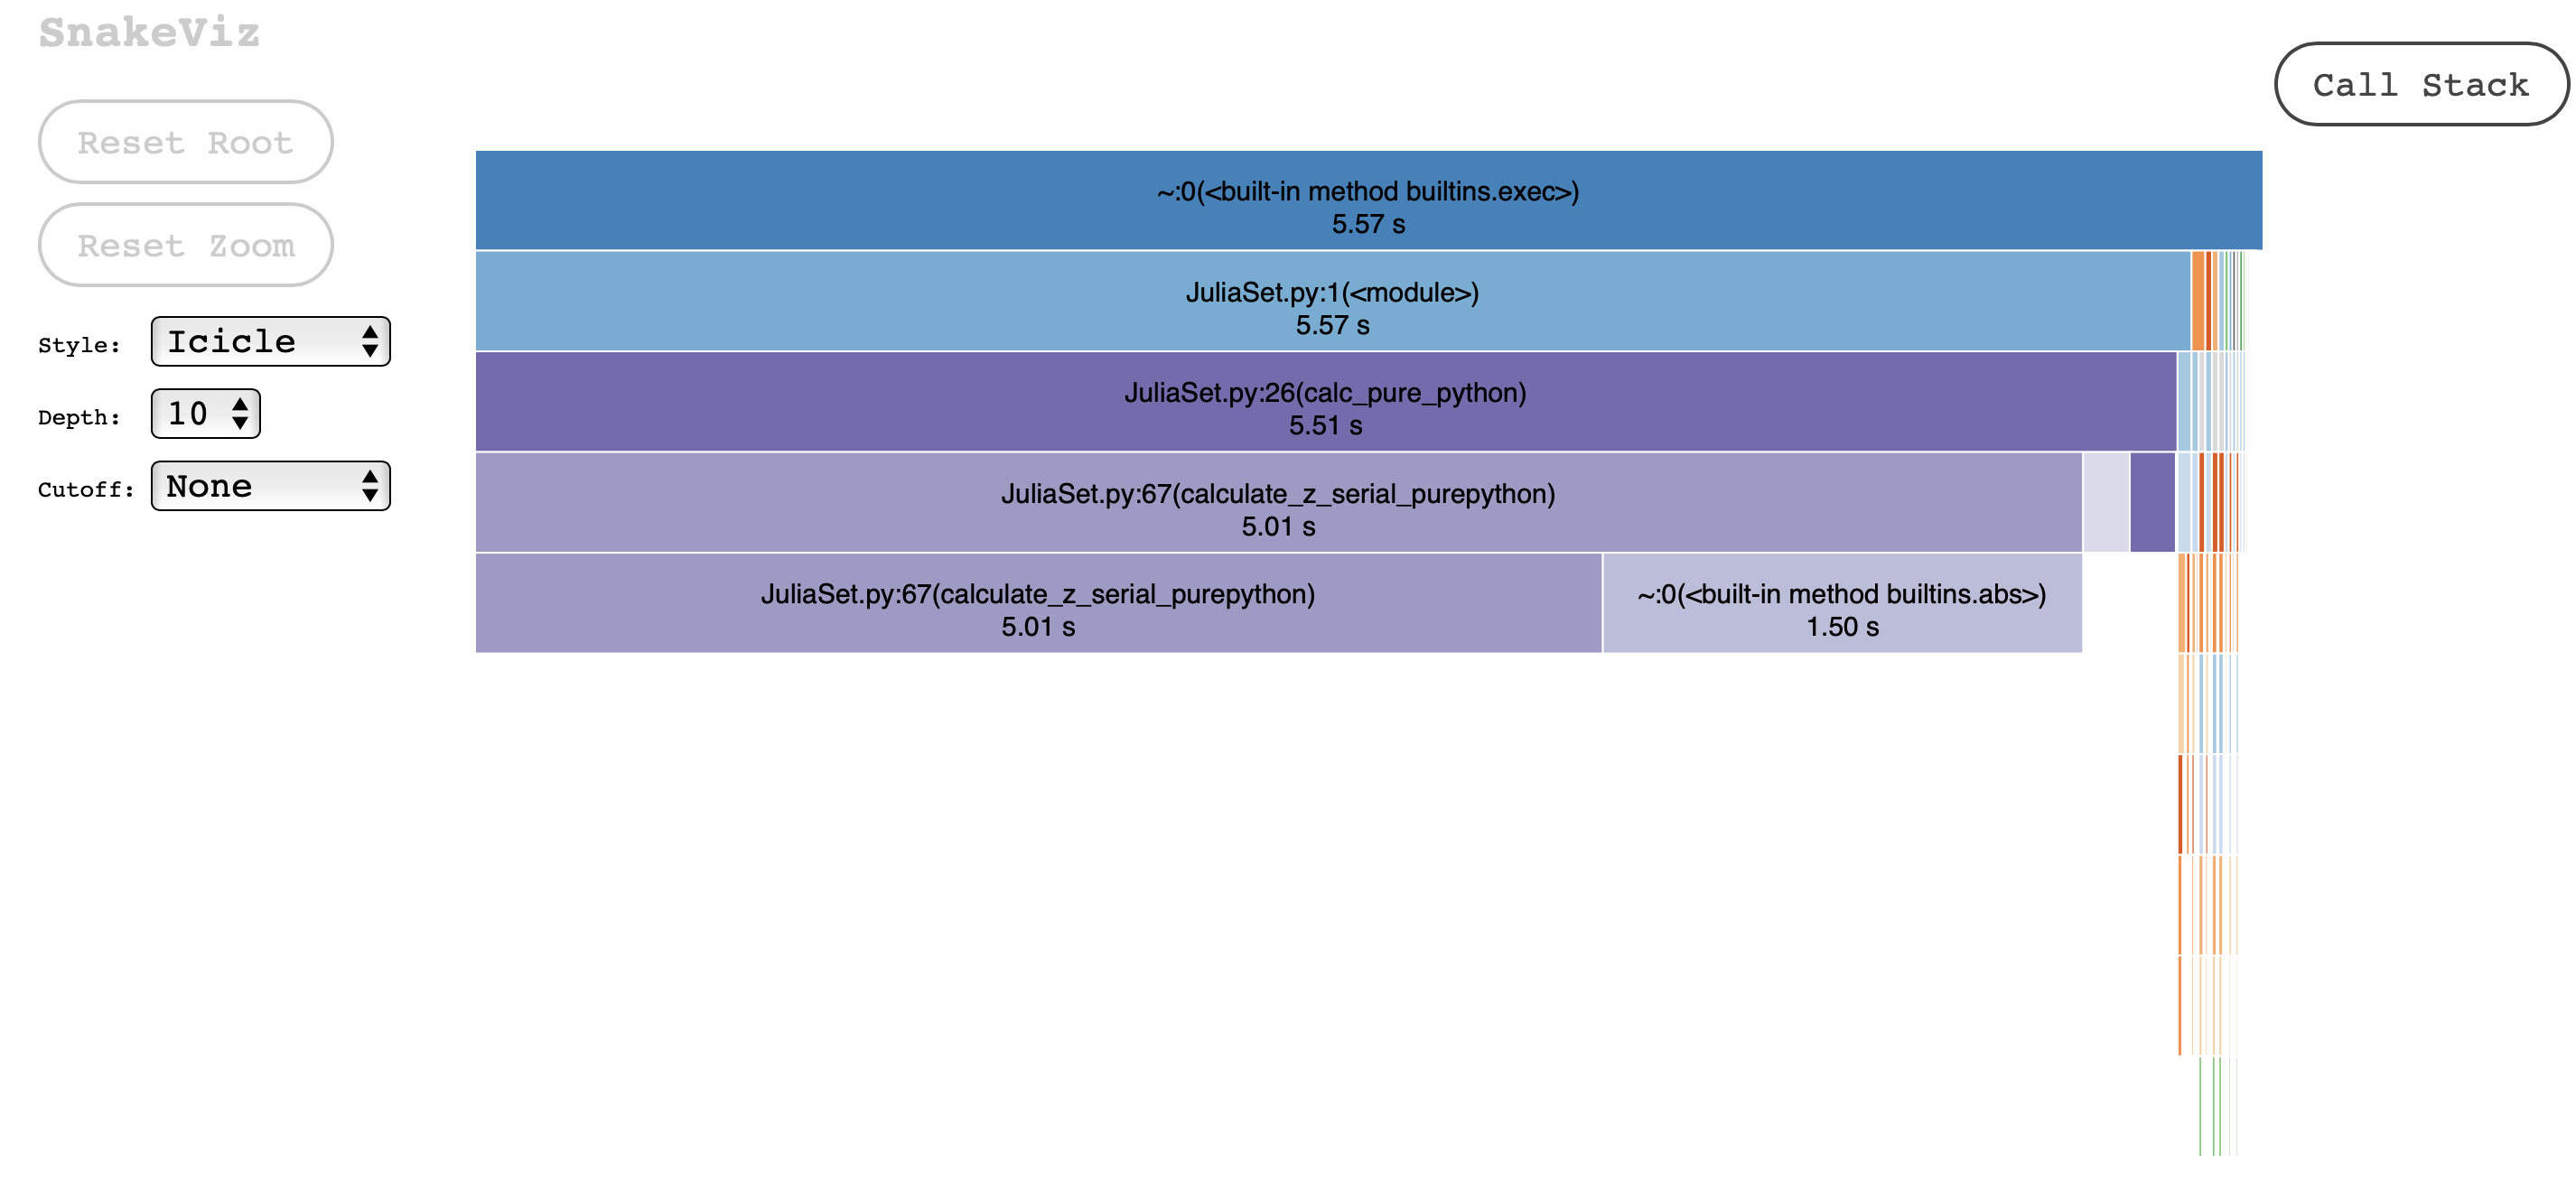
\includegraphics[width=\textwidth]{images/julia_snakeviz_view}
  \caption{Julia snakeviz view}
  \label{fig:julia-snakeviz}
\end{figure}

\textbf{Overhead:}
Running the \verb|JuliaSet| program without the profiler took $2.5 s$.
The overhead for using the \verb|cProfile| module were around 3 seconds slower.
That is over twice the runtime.

Results were even worse when using the \verb|line_profiler|.
The total runtime was around $23 s$, which is a magnitude higher than the original code.

\subsection{Memory-profile the Juliaset code. Use the memory\_profiler and mprof to profile the computation in JuliaSet code}

\verb|mprof| gives us the following result:
\begin{figure}[h!]
  \centering
  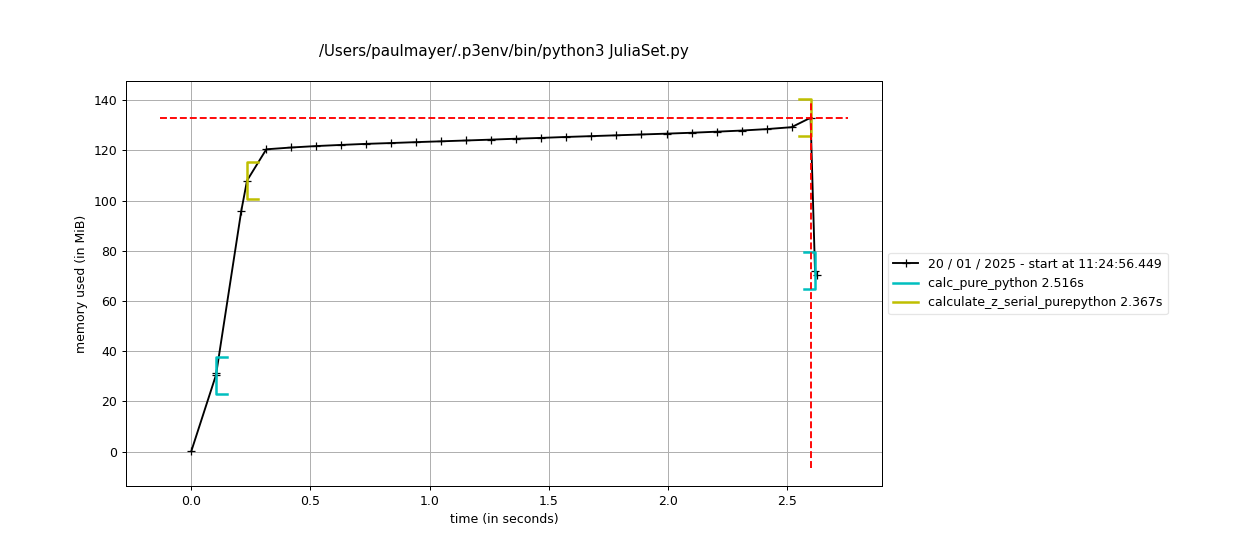
\includegraphics[width=\textwidth]{images/julia_mprofile}
  \caption{Julia mProfile}
  \label{fig:julia-mprofile}
\end{figure}

From the graph, it appears that most of the memory allocation for \verb|JuliaSet| was done in the \verb|calc_pure_python| function, as the memory usage has only a very slow increase during the execution of the \verb|calculate_z_serial_purepython| function. We can examine this further using the \verb|memory_profiler| \\

Using the line-by-line \verb|memory_profiler| returns:
\begin{lstlisting}[language=bash,basicstyle=\tiny\ttfamily]
Length of x: 100
Total elements: 10000
width:	100
output:	334236
no asserts for this dimension...
total calculation time: 15.793842832994414 s
Filename: JuliaSet.py

Line #    Mem usage    Increment  Occurrences   Line Contents
=============================================================
    25   29.625 MiB   29.625 MiB           1   @profile

    [...]

    47   30.328 MiB    0.000 MiB         101       for ycoord in y:
    48   30.328 MiB    0.016 MiB       10100           for xcoord in x:
    49   30.328 MiB    0.062 MiB       10000               zs.append(complex(xcoord, ycoord))
    50   30.328 MiB    0.625 MiB       10000               cs.append(complex(c_real, c_imag))
    51
    52   30.344 MiB    0.016 MiB           1       print("Length of x:", len(x))
    53   30.344 MiB    0.000 MiB           1       print("Total elements:", len(zs))
    54   30.531 MiB   30.531 MiB           1       output = calculate_z_serial_purepython(max_iterations, zs, cs)
    55   30.531 MiB    0.000 MiB           1       print(f"width:\t{desired_width}\noutput:\t{sum(output)}")

    [...]


Filename: JuliaSet.py

Line #    Mem usage    Increment  Occurrences   Line Contents
=============================================================
    66   30.344 MiB   30.344 MiB           1   @profile
    67                                         def calculate_z_serial_purepython(maxiter, zs, cs):
    68                                             """Calculate output list using Julia update rule"""
    69   30.453 MiB    0.109 MiB           1       output = [0] * len(zs)
    70   30.531 MiB    0.000 MiB       10001       for i in range(len(zs)):
    71   30.531 MiB    0.016 MiB       10000           n = 0
    72   30.531 MiB    0.000 MiB       10000           z = zs[i]
    73   30.531 MiB    0.000 MiB       10000           c = cs[i]
    74   30.531 MiB    0.016 MiB      344236           while abs(z) < 2 and n < maxiter:
    75   30.531 MiB    0.016 MiB      334236               z = z * z + c
    76   30.531 MiB    0.031 MiB      334236               n += 1
    77   30.531 MiB    0.000 MiB       10000           output[i] = n
    78   30.531 MiB    0.000 MiB           1       return output
\end{lstlisting}


\textbf{Overhead:}
Running \verb|mprof| did not show any significant overhead compared to unprofiled code.
However, running \verb|memory_profiler| increased the runtime by a shocking factor of $750$.

\newpage
\section{Profiling Diffusion Process Code}
\subsection{Profile the diffusion code with cProfile and line\_profiler the computation}

Using cProfile turned out to be not very insightful.
As expected, most of the time was spent in the \verb|evolve| method of the program; however, there was not much else insight we could draw from that.

\begin{figure}[h!]
  \centering
  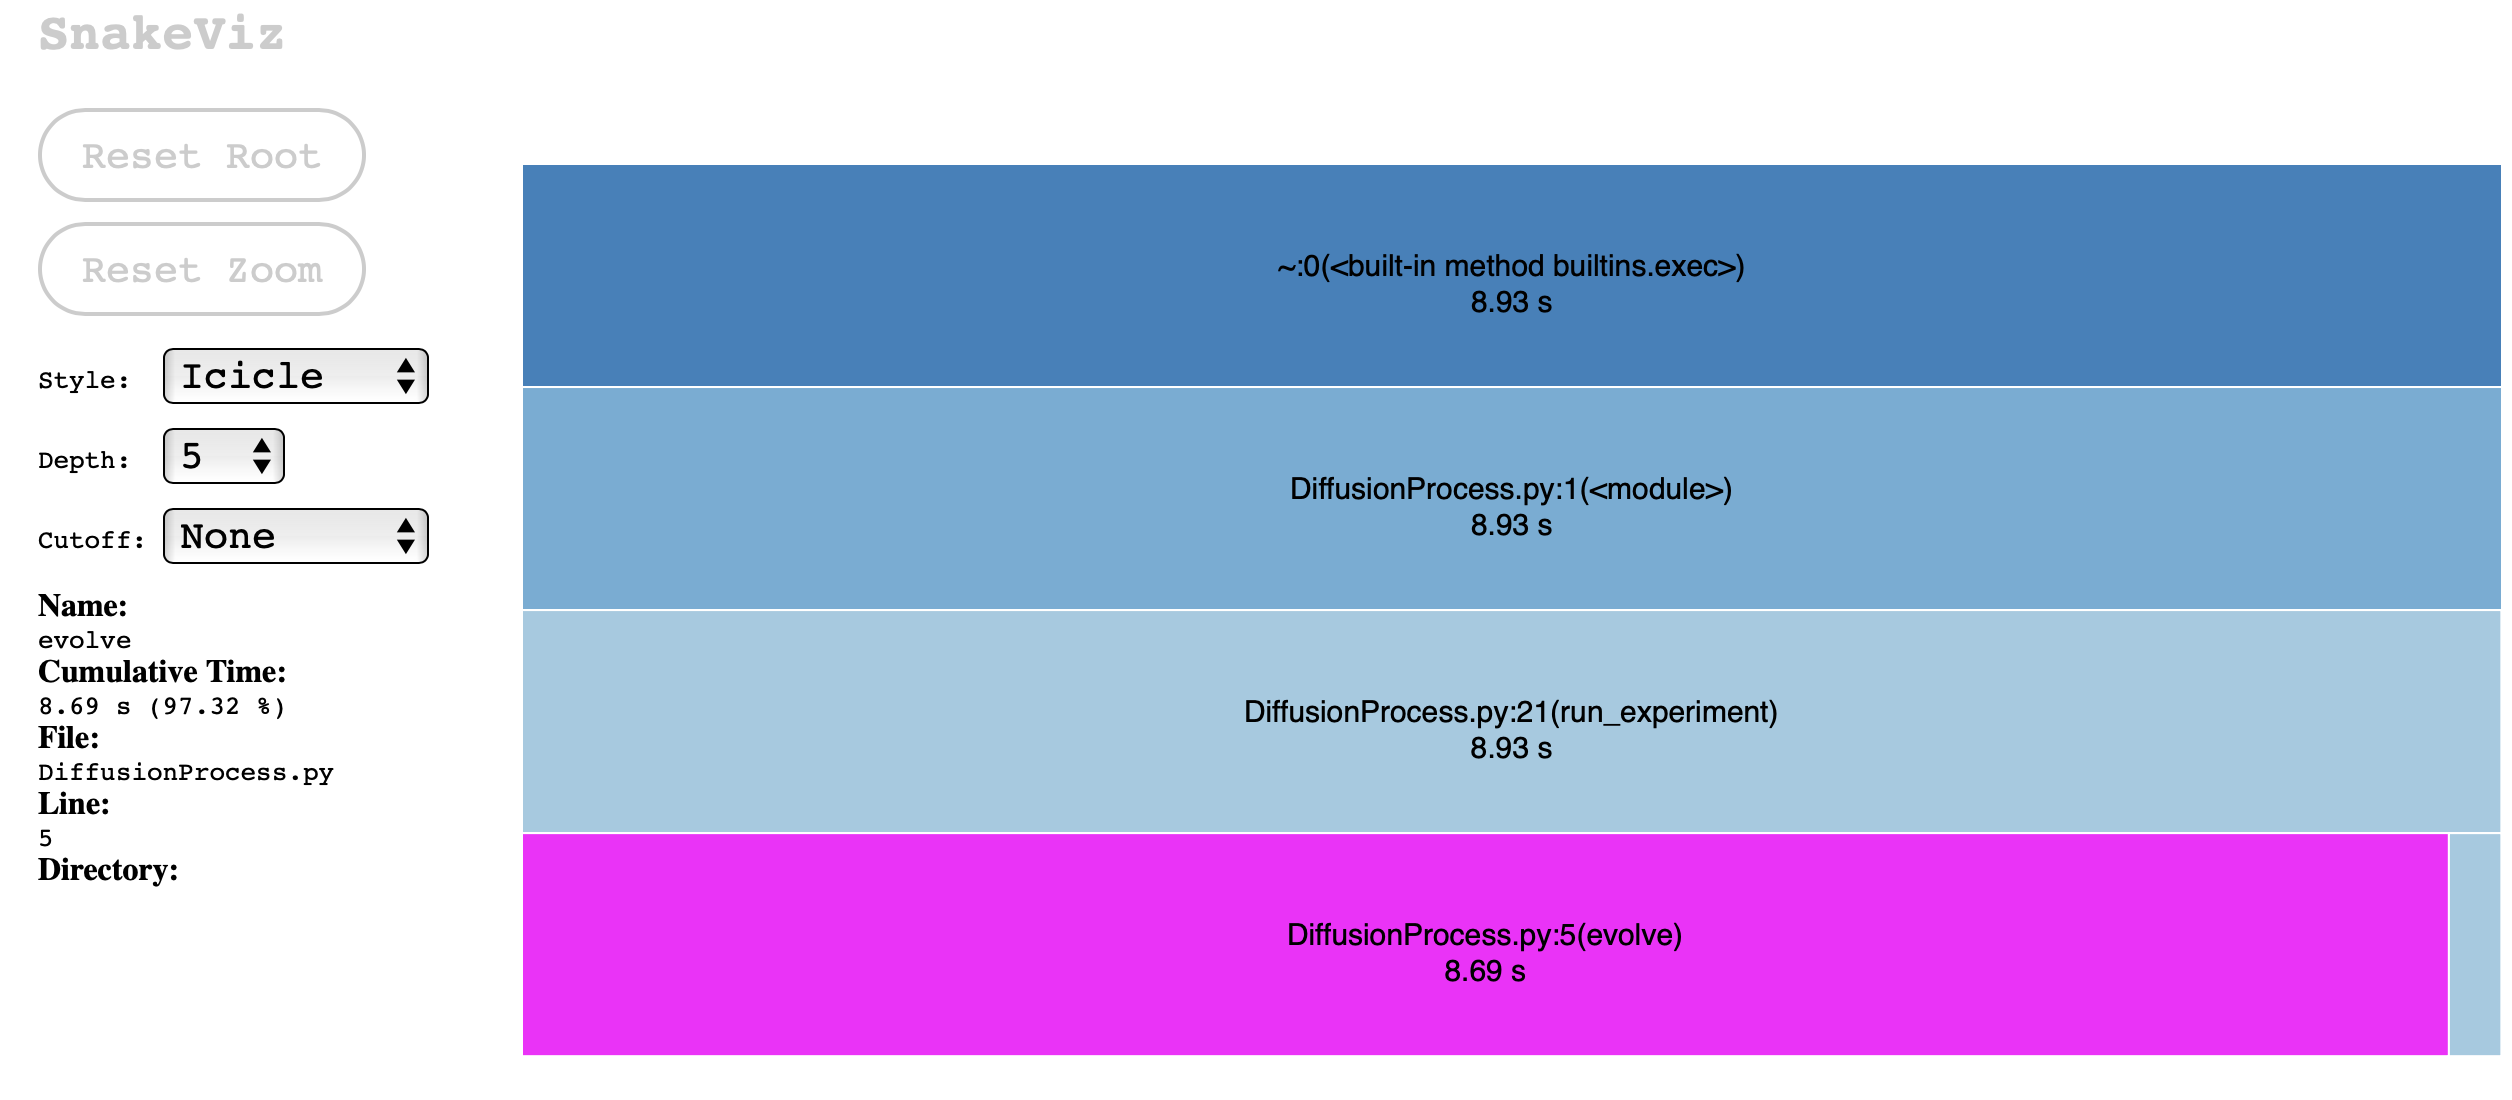
\includegraphics[width=\textwidth]{images/diffusion_snakeviz_view}
  \caption{Diffusion processing snakeviz view}
  \label{fig:diffusion-snakeviz}
\end{figure}

When diving deeper into the \verb|evolve| method using the \verb|line_profiler|, we see the following:

\begin{lstlisting}[language=bash,basicstyle=\tiny\ttfamily]
Timer unit: 1e-06 s

Total time: 29.5351 s
File: DiffusionProcess.py
Function: evolve at line 4

Line #      Hits         Time  Per Hit   % Time  Line Contents
==============================================================
     4                                           @profile
     5                                           def evolve(grid, dt, D=1.0):
     6       100         83.0      0.8      0.0      xmax, ymax = grid_shape
     7     64100      33649.0      0.5      0.1      new_grid = [[0.0] * ymax for x in range(xmax)]
     8     64100       7771.0      0.1      0.0      for i in range(xmax):
     9  41024000    4381699.0      0.1     14.8          for j in range(ymax):
    10  40960000    3618998.0      0.1     12.3              grid_xx = (
    11  40960000    6772659.0      0.2     22.9                  grid[(i + 1) % xmax][j] + grid[(i - 1) % xmax][j] - 2.0 * grid[i][j]
    12                                                       )
    13  40960000    3692418.0      0.1     12.5              grid_yy = (
    14  40960000    6465938.0      0.2     21.9                  grid[i][(j + 1) % ymax] + grid[i][(j - 1) % ymax] - 2.0 * grid[i][j]
    15                                                       )
    16  40960000    4561813.0      0.1     15.4              new_grid[i][j] = grid[i][j] + D * (grid_xx + grid_yy) * dt
    17       100        111.0      1.1      0.0      return new_grid

 29.54 seconds - DiffusionProcess.py:4 - evolve
\end{lstlisting}

Non surprisingly, calculating the grid values takes the most amount of time.
However, around 25\% of the total time spent was used to store the grid values, which seems high.

\subsection{Memory-profile the diffusion code. Use the memory\_profiler and mprof to profile the computation}

\verb|memory_profiler| (one iteration):
\begin{lstlisting}[language=bash,basicstyle=\tiny\ttfamily]
Filename: DiffusionProcess.py

Line #    Mem usage    Increment  Occurrences   Line Contents
=============================================================
     4   25.219 MiB   25.219 MiB           1   @profile
     5                                         def evolve(grid, dt, D=1.0):
     6   25.219 MiB    0.000 MiB           1       xmax, ymax = grid_shape
     7   28.391 MiB    3.172 MiB         641       new_grid = [[0.0] * ymax for x in range(xmax)]
     8   41.016 MiB    0.000 MiB         641       for i in range(xmax):
     9   41.016 MiB    0.094 MiB      410240           for j in range(ymax):
    10   41.016 MiB   12.469 MiB      409600               grid_xx = (
    11   41.016 MiB    0.016 MiB      409600                   grid[(i + 1) % xmax][j] + grid[(i - 1) % xmax][j] - 2.0 * grid[i][j]
    12                                                     )
    13   41.016 MiB    0.016 MiB      409600               grid_yy = (
    14   41.016 MiB    0.016 MiB      409600                   grid[i][(j + 1) % ymax] + grid[i][(j - 1) % ymax] - 2.0 * grid[i][j]
    15                                                     )
    16   41.016 MiB    0.016 MiB      409600               new_grid[i][j] = grid[i][j] + D * (grid_xx + grid_yy) * dt
    17   41.016 MiB    0.000 MiB           1       return new_grid
\end{lstlisting}\vspace{1em}

By using \verb|memory_profiler| we observe that most of memory usage occurs during writing the immediate variables. 
We believe that this the memory increase for the variable \verb|grid_yy| is already anticipated during the allocation
of \verb|grid_xx|. 
\verb|mprof| (10 iterations):
\begin{figure}[h!]
  \centering
  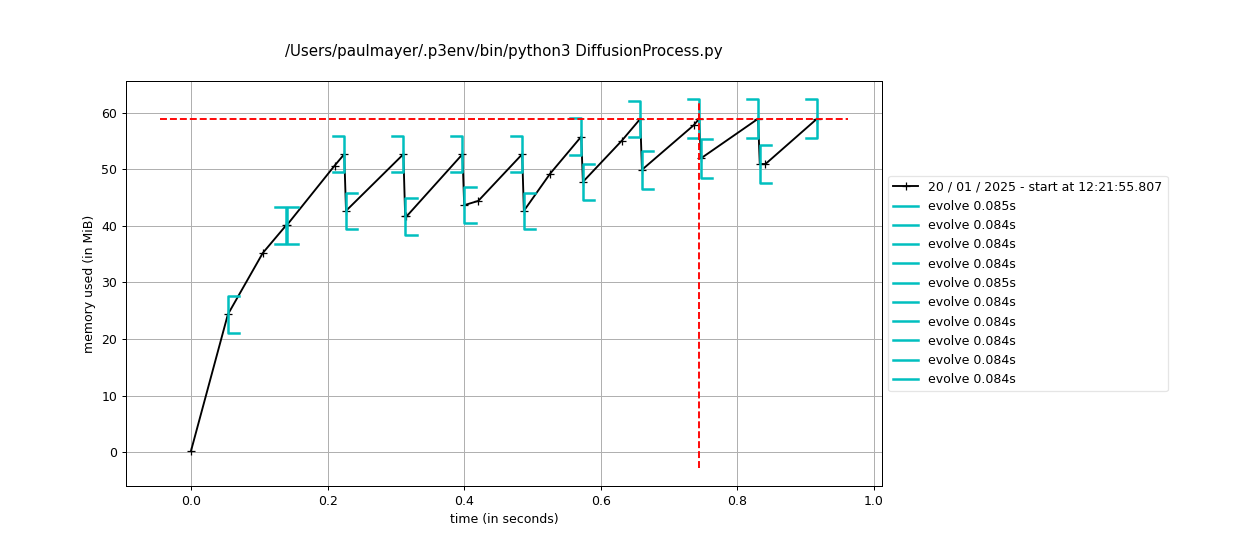
\includegraphics[width=\textwidth]{images/diffusion_mprofile}
  \caption{Diffusion mprof plot}
  \label{fig:diffusion-mprof}
\end{figure}

As for the \verb|mprof| profiling over 10 runs, we observe an asymptotic increase of memory usage. 
We assume this behavior can be explained due to the garbage collection being carried out.

\newpage
\section{Develop your profiler tool for monitoring CPU percentage use with psutil}
\subsection{Design of the profiler tool}
Our basic idea in the implementation of the profiling tool was to call the \verb|cpu_percent()| function of the \verb|psutil| library at regular intervals of time: where the intended calling frequency would be specified by the user. The profiler would then call this function until the code to profile is executing. We would determine when the code to be profiled has finished executing based on a call to a demarcation function related to the profiler. 

Since we allow the user to specify how frequently during the execution of the code they want the CPU usage percentage to be determined, we also allow the user to specify the \verb|interval| for which the usage percentage is to be monitored \textit{on each call} to \verb|psutil.cpu_percent|. This \verb|interval| provided by the user would be used as the \verb|interval| argument of the \verb|cpu_percent| function, more information on which can be found \href{https://psutil.readthedocs.io/en/latest/#psutil.cpu_percent}{here}.

Once the profiling has been completed, the user can then generate a graph showing the evolution of the usage percentages of the different CPU Cores in increments of time provided by the user at the time of initialization of the profiler. Additionally, to get more exact data in the form of tabular information printed to the screen, users can call a separate function: which will print the CPU Usage percentage per core over time, along with summary statistics: the average usage percentage per core over the course of the experiment, and the standard deviation in this usage percentage.

\subsection{Implementation of the profiler tool}
The implementation of the profiling tool can be found in the \verb|cpuprofiler.py| file of the GitHub repo for the assignment, located \href{https://github.com/paulmyr/DD2358-HPC25/blob/master/01_profiling/cpuprofiler.py}{here}. 

We have implemented our profiling tool in a class called the \verb|CPUProfiler|. Since we allow the user to specify the granularity of the measurements (ie, how frequently through the course of the experiment the core usage is to be recorded) and the \verb|interval| argument to be passed to \verb|cpu_interval|, implementing the tool through a class felt the best way to preserve this and some other useful state. The class has 4 usable methods: \verb|initiate_observation|, \verb|end_observation|, \verb|generate_usage_graph|, \verb|generate_tabular_summary|.

The \verb|initiate_observation| function spawns a separate thread which, at the frequency specified by the user during object instantiation, calls the \verb|cpu_percent| method and stores the results in an interval data structure. The \verb|interval| argument passed to the \verb|cpu_percent| method is the same as the \verb|interval| value specified by the user at object instantiation. This is done until the code to be profiled has finished execution. 

The \verb|end_observation| method is responsible for stopping the profiling of the experiment code. Thus, this marks as the barrier which indicates to \verb|CPUProfiler| that the code being profiled has finished, and thus the periodic calls to \verb|cpu_percent| by \verb|initiate_observation| can end. This is done through a flag, whose value is changed by \verb|end_observation|.

The \verb|generate_usage_graph| function is responsible for generating a plot of the CPU Core usage percentage over the course of the experiment. The \textit{x-}axis marks the elapsed time (in seconds), and the \textit{y-}axis marks the usage percentage. There is 1 line in the graph for each core on the system.

The \verb|generate_tabular_summary| function is responsible for printing tabular information about the cpu usage of the profiled code to the screen. This prints fine-grained information: which is the usage-percentage for each core at each point of time (in terms of \textit{elapsed time} since measurement began) the usage was recorded, and it prints coarse-grained information: which is the mean usage-percentage and standard deviation for each core while the profiled code was being executed. We use the \verb|tabulate| library to help with the table generation. 

Currently, we enforce that the \verb|granularity >= interval| at the time the \verb|CPUProfiler| is being created. This is because \verb|cpu_percent| is a blocking call, and some complications arise in the case when the execution of code in the monitoring thread (spawned by \verb|initiate_observation|) takes longer to execute than the points in time when observations are to be made. 

The code provides more information on implementation and example usage through comments and docstrings.

\subsection{Results}
We profiled the \verb|JuliaSet| code and the \verb|DiffusionProcess| code using the function called \verb|do_cpu_usage_estimation| present in each file. For each of these measurements, we used the \verb|CPUProfiler| with \verb|granularity| set to 5 seconds and \verb|interval| set to 1 second. The Profiling was done on a 2021 MacBook Pro with Apple's M1 Chip, which has 10 CPU Cores. 

For the \verb|JuliaSet| code, we profiled the call to \verb|calc_pure_python| with \verb|desired_width| set to 5000 and \verb|max_iterations| set to 300. On doing so, we got the following plot (through \verb|generate_usage_graph|)

\begin{figure}[h!]
  \centering
  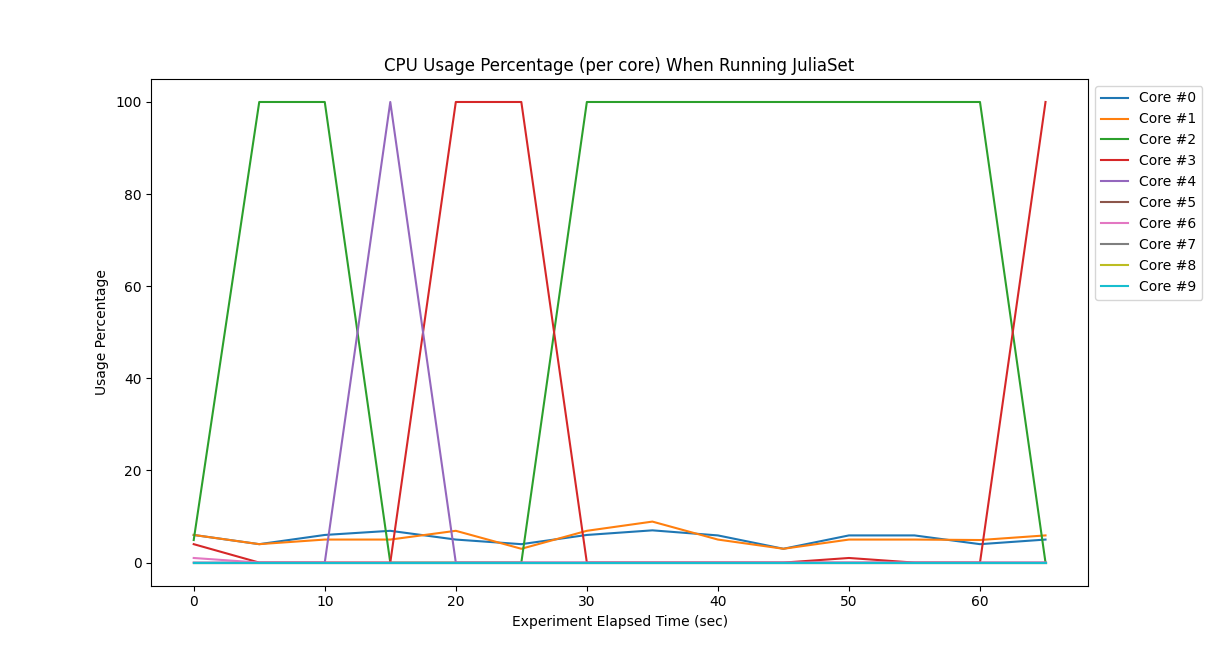
\includegraphics[width=\textwidth]{images/cpuprofile_juliaset.png}
  \caption{CPU Usage Percentage Per Core for JuliaSet}
  \label{fig:cpuprofiler_julia}
\end{figure}

The \verb|generate_tabular_summary| function generated tabular output which can be found in the repository \href{https://github.com/paulmyr/DD2358-HPC25/blob/master/01_profiling/outputs/cpuprofile_juliaset.output}{here} (copy-pasting the output proved to be difficult, as it contained encoding that wasn't easily recognized by \LaTeX). 

For the \verb|DiffusionProcess| code, we profiled the call to \verb|run_experiment| with \verb|num_iterations| being 500. On doing so, we got the following plot (through the function \verb|generate_usage_graph|)

\begin{figure}[h!]
  \centering
  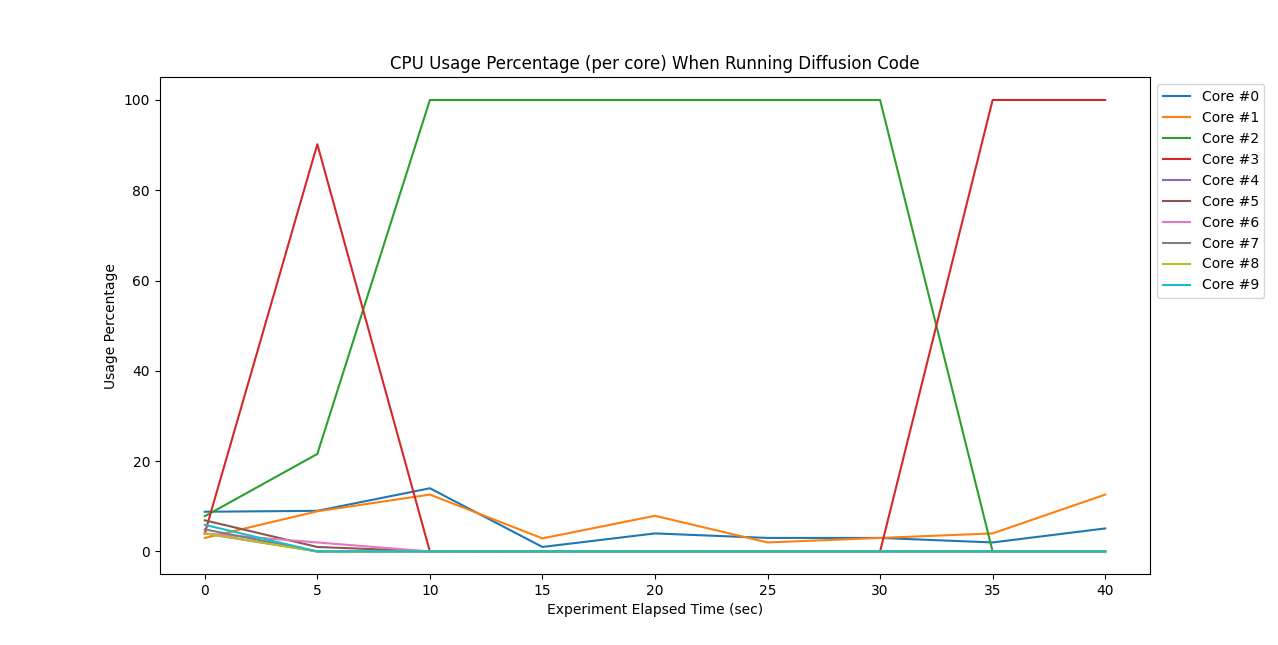
\includegraphics[width=\textwidth]{images/cpuprofile_diffusion.png}
  \caption{CPU Usage Percentage Per Core for DiffusionProcess}
  \label{fig:cpuprofiler_diffusion}
\end{figure}

The \verb|generate_tabular_summary| function generated tabular output which can be found in the repository \href{https://github.com/paulmyr/DD2358-HPC25/blob/master/01_profiling/outputs/cpuprofile_diffusion.output}{here} (as above, copy-pasting proved to be difficult in \LaTeX). 

\subsection{Discussion}
We shall now briefly attempt to draw some conclusions from the result of the profiling above. 

We would like to first mention that the presence of multiple cores and of background applications running on the machine makes it rather difficult to discern clearly observable evolution patterns in the impact of the code being profiled on CPU Usage: since the same process could go from being executed on one core to another (because of CPU Interrupts, for instance), and other processes could add to some noise in the observed usage percentages for the different cores. Nevertheless, we shall make our best attempt to deduce some findings. 

Looking at the results for \verb|JuliaSet|, it seems evident that Cores 2, 3, and 4 seem to have been the most busy at different points in time during the course of the experiment. It thus seems plausible to hypothesize that these 3 cores could have been the ones being used in the computation at different periods of time. Of these 3 cores, Core 2 seems to be the most busy for the longest period of time. Thus, we believe that Core 2 could have been running the JuliaSet computation for the longest. The other cores seem to have minimal activity on them, which could mean that they were only being used by other processes while the experiment was being profiled.

A similar pattern can be seen in the results for the \verb|DiffusionProcess| code. Here, Cores 2 and 3 seem to be the most busy over the time the experiment was being profiled. An interesting pattern can be seen at elapsed time 10sec and elapsed time 35sec. At 10sec, the busiest Core seems to switch from 2 to 3, and the reverse happens at 35sec. This could mean that the CPU switched the core on which the computation was being run when between the observations made at 5sec and 10sec, and the observations made at 30sec and 35sec. Of these 2 cores, it seems Core 2 was responsible for computation for the most amount of time. Like with the \verb|JuliaSet| results, it appears that the other cores had little to no involvement in the computation. 


% content end
%###############################################################################

% TODO: bibliograpghy when needed
% \printbibliography

\end{document}
